\section{Optimization Framework}

%\setbeamercovered{transparent}
\begin{frame}[t]
\frametitle{Proposed Solution}
\framesubtitle{General Idea}

\begin{itemize}
	\item<1-> Explore the hyperparameter space of model learning algorithms
	\item<2-> Use \textit{Bayesian Optimization} to sequentially sample hyperparameter~settings $\theta$ towards a global maximizer of a performance measure of learned MDPs
\end{itemize}

\begin{center}
	%\includegraphics<-2|handout:0>[width=\textwidth]{figures/bo_toy_example_v2_transparent}
	\includegraphics<3->[width=\textwidth]{figures/bo_toy_example_two_iterations}
\end{center}

\end{frame}
%\setbeamercovered{invisible}

\begin{frame}
\frametitle{Proposed Solution}
\framesubtitle{Running Example: Path Planning for Mobile Robot Navigation}

\centering
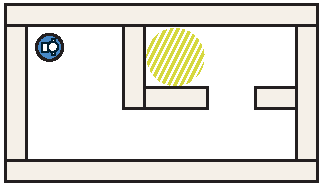
\includegraphics[width=.3\textwidth]{figures/dummy-map-2-1}
\qquad
\includegraphics<-1| handout:0>[width=.3\textwidth]{figures/dummy-map-2-2-transparent}
\includegraphics<2->[width=.3\textwidth]{figures/dummy-map-2-2v2}\\\vspace{8pt}
\includegraphics<-2| handout:0>[width=.3\textwidth]{figures/dummy-map-2-3-transparent}
\includegraphics<3->[width=.3\textwidth]{figures/dummy-map-2-3} \qquad
\includegraphics<-3| handout:0>[width=.3\textwidth]{figures/dummy-map-2-4-transparent} \includegraphics<4->[width=.3\textwidth]{figures/dummy-map-2-4}


\end{frame}

\begin{frame}
\frametitle{Proposed Solution}
\framesubtitle{Performance Measure}
\begin{itemize}
	\item<1-> \footnotesize Performance is assessed over multiple tasks $T$ (each mappable to a pair $(s_0, R)$)
	\item<2-> Based on Value Functions from DTP algorithm (e.g., VI, PI):
	$$V_{\mathit{DTP}, (s_0, R)} = V[s_0]$$
	\item<3-> Based on Simulations:
	$$V_{\mathit{SIM}, (s_0, R)} = \gamma^n \cdot R[i]$$
	\item<4-> Combined:
	$$V_{\mathcal{M}} = \frac{\sum_{t \in T_\mathcal{M}} \beta \cdot V_{\mathit{DTP}, t} + (1 - \beta) \cdot V_{\mathit{SIM}, t}}{|T_\mathcal{M}|}$$
%	% Level of abstraction
%	\item Value Function
%	\item Simulations
%	
%	\item Lorem ipsum dolor sit amet
%$$V_{\mathcal{M}} = \frac{\sum_{t \in T_\mathcal{M}} \beta \cdot V_{\mathit{DTP}, t} + (1 - \beta) \cdot V_{\mathit{SIM}, t}}{|T_\mathcal{M}|}$$
\end{itemize}

\end{frame}

\begin{frame}
\frametitle{Proposed Solution}
\framesubtitle{Base Framework}
	\vspace{-10pt}
	\begin{center}
		\includegraphics<1| handout:0>[width=1\textwidth]{figures/optimization-routine/learning-cycle-simplified-1.pdf}
		\includegraphics<2| handout:0>[width=1\textwidth]{figures/optimization-routine/learning-cycle-simplified-2.pdf}
		\includegraphics<3>[width=1\textwidth]{figures/optimization-routine/learning-cycle-simplified-3.pdf}
	\end{center}
\end{frame}

\begin{frame}
\frametitle{Proposed Solution}
\framesubtitle{Multi-Phase Framework: Phase 1}

\begin{center}
	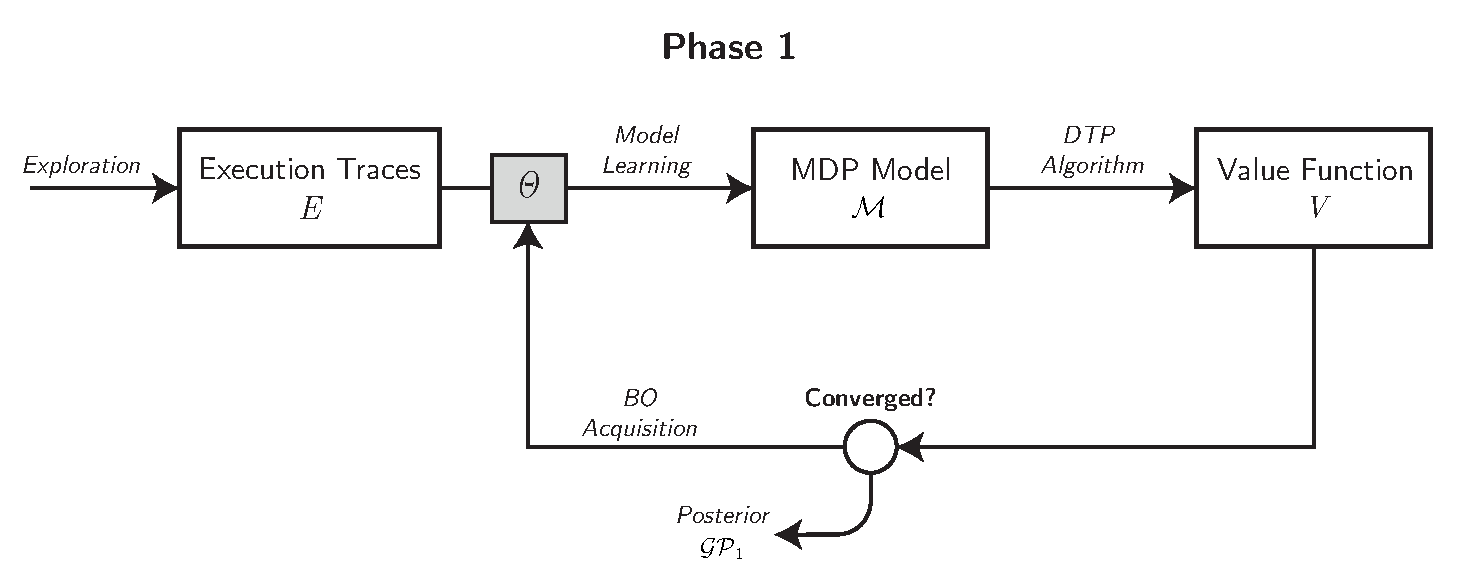
\includegraphics[width=\textwidth]{figures/phase-1v2}
\end{center}

\end{frame}

\begin{frame}
	\frametitle{Proposed Solution}
	\framesubtitle{Multi-Phase Framework: Phase 2}
	
	\begin{center}
		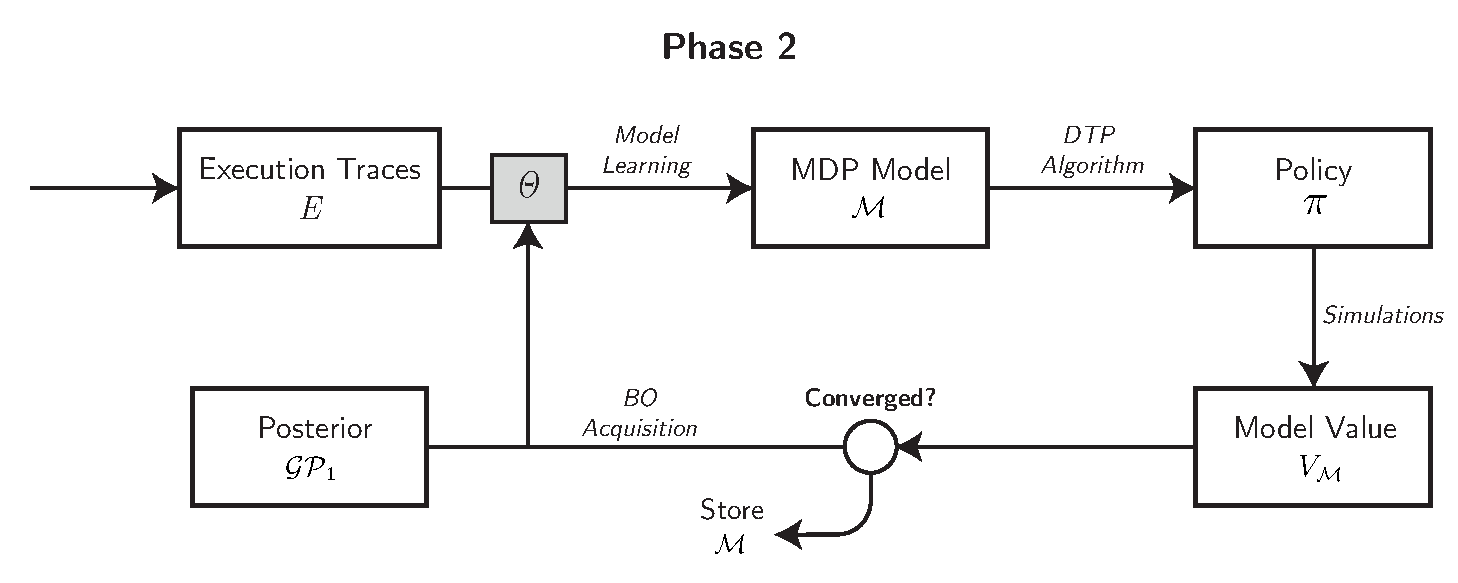
\includegraphics[width=\textwidth]{figures/phase-2v3}
	\end{center}
	
\end{frame}

\begin{frame}
	\frametitle{Proposed Solution}
	\framesubtitle{Multi-Phase Framework: Phase 3}
	
	\begin{center}
		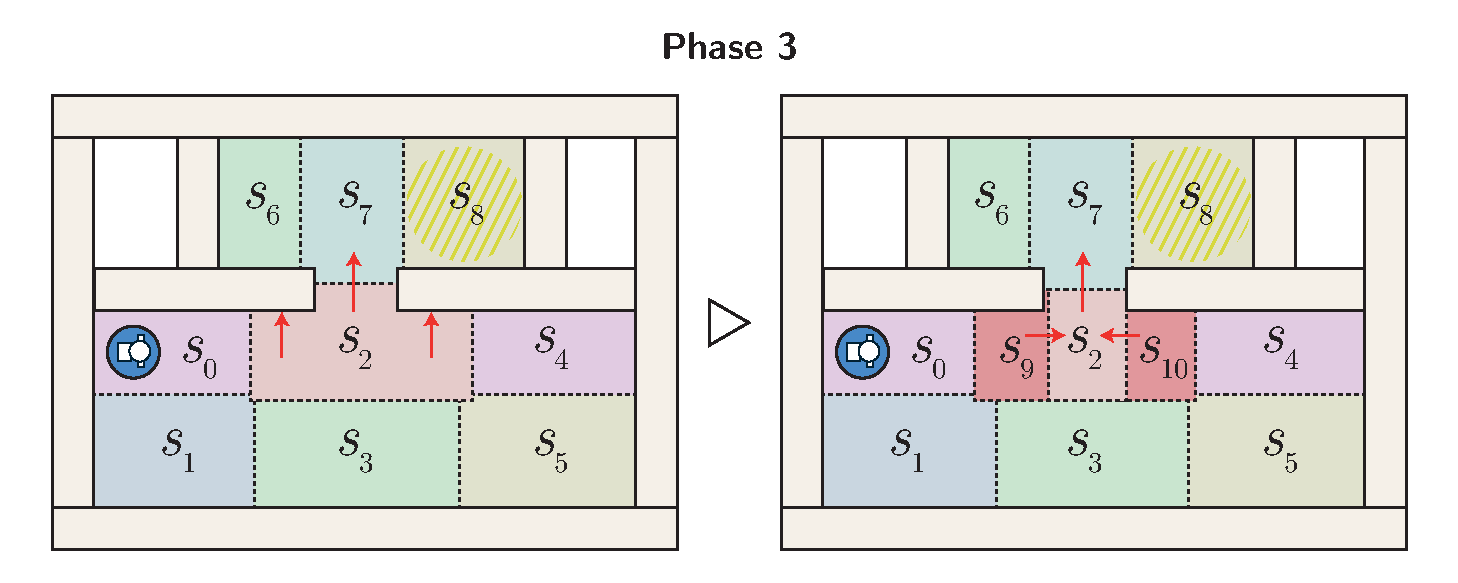
\includegraphics[width=\textwidth]{figures/phase-3}
	\end{center}
	
\end{frame}